\chapter{Bases biol\'ogicas del c\'ancer}\label{chapter:proposal}

\hspace{.1cm}La neoplasia (en griego, ``nuevo crecimiento``) es el proceso de proliferación descontrolada de células en un tejido, el cual por sus características histológicas o inclusive genéticas, puede ser benigno o maligno. El término tumor, que en un principio se aplicó a la tumefacción causada por la inflamación, actualmente se equipara al de neoplasia \cite{robins}. El conjunto de mutaciones sufridas por las células pertenecientes a la neoplasia determinan el estado del desarrollo de la enfermedad y la transición entre sus etapas ocurre cuando dichas células adquieren mutaciones específicas que le hacen ganar malignidad. Es decir, el desarrollo tumoral está sujeto a la obtención de dichas mutaciones por las células que lo conforman. En esta sección se caracterizan las etapas del desarrollo del cáncer a partir del proceso de acumulación de mutaciones de las células cancerígenas y las capacidades que adquieren \cite{viabarre2019}.

\section{La célula cancerígena}
\hspace{.1cm}Las células cancerígenas se comportan de forma distinta a las células normales. En la mayoría de los casos el cáncer se produce por la aparición de mutaciones genéticas (en la secuencia de ADN) o epigenéticas (en mecanismos que influyen en la regulación de los genes sin afectar a la secuencia de ADN) en genes de susceptibilidad al cáncer. Las mutaciones en el código genético traen como consecuencia defectos en la regulación del ciclo vital de la célula, que interrumpen su proliferación normal. Pero no se trata de cualquier tipo de mutación, sino de mutaciones específicas: unas que llevan a que las células pierdan el control del ciclo celular y puedan empezar a ganar características biológicas que favorezcan su supervivencia.
Entre estas características destacan:
\begin{itemize}
    \item La capacidad energética para mantener una proliferación continuada: Las células tumorales son células con grandes requerimientos energéticos así que deben adaptarse a obtener energía de donde puedan. Pueden incluso reprogramar su metabolismo, si es necesario, para adaptarse a sus nuevas necesidades.
    \item La evasión de las señales para suprimir el crecimiento: Las células tumorales no respetan los semáforos celulares que indican que es el momento de detener el crecimiento.
    \item Capacidad para evadir la muerte celular programada (apoptosis) y no verse afectadas por las múltiples divisiones. Normalmente, las células tienen una suerte de ``obsolescencia programada``, un número límite de divisiones que pueden tolerar antes de que se produzcan alteraciones en sus cromosomas. Cuando llega ese momento y en otras situaciones de estrés, las células activan programas de muerte celular programada como medida de control para evitar que la acumulación de daños pueda repercutir en el funcionamiento o generar problemas a otras células. Las células del cáncer consiguen evitar esos programas y se adaptan a las múltiples divisiones.
    \item Capacidad para inducir la formación de vasos sanguíneos (angiogénesis), por donde pueden obtener nutrientes o establecer vías para invadir otros tejidos e iniciar lo que se conoce como metástasis.
    \item Evasión de la acción del sistema inmunitario, algo esencial para no ser reconocidas como perjudiciales (son células sin control) y ser eliminadas.
    \item Inmortalidad replicativa y la capacidad de esparcirse a otras localizaciones (metástasis) \cite{genotipia2024}.
\end{itemize}

\hspace{.1cm}La obtención de estas mutaciones distintivas es un proceso continuo, consecuencia de una acumulación de errores en el código genético que ocurre en la célula cancerígena [\cite{invasion}, \cite{cancerbook}]. La primera célula cancerígena no surge cuando aparece una sola mutación, sino cuando este proceso de acumulación crea una célula que contiene todas las mutaciones que caracterizan al cáncer. Un grupo importante de estas mutaciones son las relacionadas con los genes que mantienen la estabilidad genómica. Si los genes que codifican las proteínas encargadas de reparar el código genético y llevar a cabo varias funciones de mantenimiento del genoma son afectados por una mutación, haciendo que pierdan en alguna medida su correcto funcionamiento, otras mutaciones pueden acumularse mucho más rápido \cite{robins}. Un ejemplo de este proceso de acumulación se aprecia en la figura~(Fig.\ref{fig-evolution}).

% \captionsetup{justification=centering}
\begin{figure}[!ht]
    \begin{center}
    \scalebox{0.75}{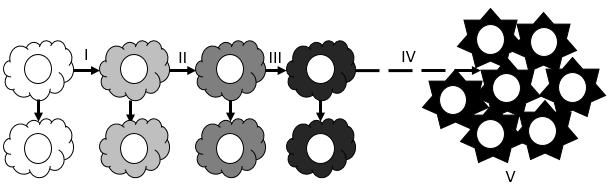
\includegraphics{img/fig-evolution.png}}
    \end{center}\vspace*{-0.6cm}
    \caption[Proceso de acumulaci\'on de mutaciones que provocan la aparici\'on del c\'ancer]{Proceso de acumulaci\'on de mutaciones que provocan la aparici\'on del c\'ancer~\cite{robins}. Las mutaciones sufridas por las poblaciones de c\'elulas y sus descendientes son las siguientes: aparece una mutaci\'on inicial que desactiva un inhibidor del ciclo celular~(\emph{I}); la c\'elula mutada contin\'ua su divisi\'on y un descendiente adquiere una nueva mutaci\'on que activa un estimulante del ciclo celular~(\emph{II}); el proceso contin\'ua y aparece una c\'elula con una nueva mutaci\'on que desactiva un factor de estabilidad gen\'omico~(\emph{III}); las mutaciones se acumulan r\'apidamente por la p\'erdida de la estabilidad gen\'etica hasta que aparece la primera c\'elula cancer\'igena~(\emph{IV}); aparece el c\'ancer como enfermedad por la divisi\'on descontrolada de estas c\'elulas altamente mutadas~(\emph{V}) \cite{viabarre2019}.}
    \label{fig-evolution}
    \end{figure}

\section{Inmortalidad replicativa}
\hspace{.1cm}El cáncer es esencialmente una enfermedad de división celular incontrolada. Su desarrollo y progresión suelen estar vinculados a una serie de cambios en la actividad de los reguladores del ciclo celular. Por ejemplo, los inhibidores del ciclo celular evitan que las células se dividan cuando las condiciones no son las adecuadas, por lo que la reducción de la actividad de estos inhibidores puede promover el cáncer. Del mismo modo, los reguladores positivos de la división celular, pueden conducir al cáncer si son demasiado activos. En la mayoría de los casos, estos cambios en la actividad se deben a mutaciones en los genes que codifican proteínas reguladoras del ciclo celular \cite{khanacademy2024}.

\hspace{.1cm}En un cultivo las células normales pueden llevar a cabo una cantidad finita de divisiones antes de que detengan su división completamente, mientras que las células cancerígenas pueden dividirse indefinidamente. Esto ocurre porque las células poseen un número finito de posibles divisiones celulares o potencial replicativo. Una célula humana puede dividirse de 60 a 70 veces como promedio antes de que incurra en un proceso conocido como senescencia. Una célula senescente es viable pero ha perdido su capacidad de dividirse.

\hspace{.1cm}El mecanismo que se encarga de la senescencia es un contador que controla la cantidad finita de divisiones celulares y se encuentra en los extremos de todos los cromosomas del cuerpo humano: los telómeros. Los telómeros son secuencias de material genético que no codifican ninguna proteína por lo que se conoce como secuencias basura. No obstante, juegan un papel fundamental en la protección de los cromosomas. Su importancia radica en un problema único presente en la replicación del código genético durante la división celular. Después de cada ronda de replicación del código genético se pierde una corta secuencia del telómero en los extremos de cada cromosoma. Como resultado de la degradación de los telómeros los cromosomas se hacen más cortos. Los ciclos sucesivos de replicación traen como consecuencia una erosión continua de los telómeros hasta el punto en que comienzan a causar problemas en el código genético tales como cambios genéticos, errores de escritura y muerte celular. Por tanto, una célula normal posee un ciclo vital finito, dictado por la longitud de sus telómeros~(Fig.\ref{fig-telomero}) [\cite{robins}, \cite{hanahan}, \cite{cancerbook}]

\begin{figure}[!ht]
\begin{center}
\scalebox{0.75}{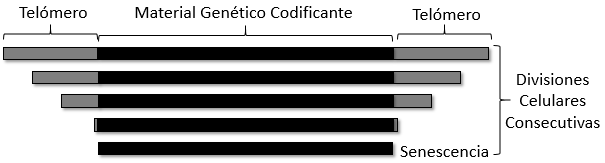
\includegraphics{img/fig-telomero.png}}
\end{center}\vspace*{-0.6cm}
\caption[Proceso de degradaci\'on de los tel\'omeros de una c\'elula]{Proceso de degradaci\'on de los tel\'omeros de una c\'elula a medida que ocurren divisiones celulares consecutivas hasta alcanzar el estado de senescencia \cite{viabarre2019}.}
\label{fig-telomero}
\end{figure}

\hspace{.1cm}Las células cancerígenas por otra parte, mantienen la longitud de sus telómeros sin la pérdida de material genético codificante. La principal estrategia utilizada para mantener la longitud de los telómeros es mediante la activación de una enzima llamada telomerasa. El 85-90\% de todas las formas de cáncer presentan la activación de telomerasa. La telomerasa mantiene la longitud de los telómeros por encima del umbral crítico, previniendo la erosión y habilitando un potencial replicativo ilimitado [\cite{robins}, \cite{hanahan}, \cite{cancerbook}]. La evidencia listada sugiere que la senescencia es un mecanismo de protección utilizado por las células para entrar en una fase inactiva que detiene su proliferación. Los tumores evitan la senescencia activando la telomerasa por lo que las estrategias terapéuticas encaminadas a inhibir la telomerasa afectará preferentemente a células cancerígenas y no al correcto funcionamiento del organismo \cite{viabarre2019}.

\section{Oncogenes}
\hspace{.1cm}Los proto-oncogenes son genes involucrados en el control del crecimiento y la división de las células sanas. Por lo general, los proto-oncogenes contienen la información genética para sintetizar:
\begin{itemize}
    \item Factores de crecimiento.
    \item Receptores de factores de crecimiento y hormonas.
    \item Transductores de señales intracelulares.
    \item Factores de transcripción nucleares.
    \item Elementos clave del control del ciclo celular.
\end{itemize}

\hspace{.1cm}La actividad normal de los proto-oncogenes es benigna y no supone ningún riesgo para la salud. Sin embargo, cuando por algún motivo se incrementa la actividad de estos genes, se transforman en oncogenes, que promueven un crecimiento y proliferación celular descontrolados.

\hspace{.1cm}Existen diversos factores que pueden provocar la mutación de los proto-oncogenes y, por tanto, su transformación a oncogenes. Algunos de los ejemplos más estudiados son la exposición a radiación y errores en la replicación del ADN durante la división celular \cite{genotipia2024}.

%(Aqui viene una imagen)
\begin{figure}[!ht]
\begin{center}
\scalebox{0.75}{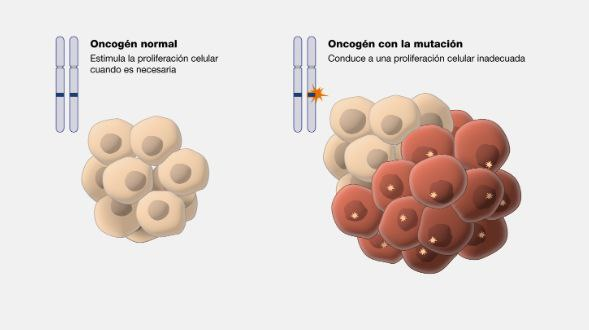
\includegraphics{img/fig-oncogen.jpg}}
\end{center}\vspace*{-0.6cm}
\caption[Imagen de Oncogenes. Falta poner leyenda]{A la izquierda, un oncogén normal, que funciona como el pedal del acelerador de un auto, estimulando la proliferación celular solo cuando es necesaria. Este oncogén juega un papel crucial en la regulación de la división celular normal, permitiendo a las células dividirse y multiplicarse de manera controlada y saludable.

Por otro lado, a la derecha, encontramos un oncogén con mutación, que se comporta más como un freno defectuoso en un auto estacionado en una colina. Esta mutación causa una proliferación celular descontrolada, llevando a una división celular excesiva y potencialmente cancerosa.}
\label{fig-oncogen}
\end{figure}
\newpage

\section{Genes supresores de tumores}
\hspace{.1cm}El balance entre la proliferación y la inactividad celular es el resultado de una compleja interacción entre los reguladores del ciclo celular: los estimulantes y los inhibidores. Como apreciamos anteriormente, los estimulantes comprenden una variedad de señales y factores de crecimiento que activan la proliferación celular. Sin embargo, los tejidos sanos también están sujetos a señales antiproliferación que son responsables de la inactividad celular, y actúan como frenos a las señales de crecimiento. Los inhibidores pueden estar presentes en la matriz extracelular (de ahora en adelante ECM) y en la superficie celular[\cite{robins}, \cite{hanahan}, \cite{cancerbook}]. De forma similar a las señales de crecimiento, las señales que bloquean o suprimen la división celular se reciben a través de receptores en la superficie de la célula y promueven o inhiben la expresión de genes específicos. Los genes que codifican esta clase de proteínas involucradas en la supresión de la división celular se conocen como genes supresores de tumores \cite{viabarre2019}.

\hspace{.1cm}Estos son genes protectores. Normalmente, limitan el crecimiento celular al:
\begin{itemize}
    \item Monitorear qué tan rápido las células se dividen en células nuevas.
    \item Reparar el ADN incompatible.
    \item Controlar cuándo una célula muere.
\end{itemize}
Cuando un gen supresor de tumor muta, las células crecen descontroladamente. Y, finalmente, pueden formar un tumor.

\hspace{.1cm}Los ejemplos de genes supresores de tumores incluyen BRCA1, BRCA2, y p53 o TP53. Las mutaciones de la línea germinal en los genes BRCA1 o BRCA2 aumentan el riesgo de una mujer de desarrollar cáncer de mama u ovarios hereditario y en el caso de un hombre de desarrollar cáncer de mama o cáncer de próstata hereditario. También aumentan el riesgo de desarrollar cáncer pancreático y melanoma en mujeres y hombres.

\hspace{.1cm}El gen con mutación más frecuente en personas con cáncer es p53 o TP53. Más del 50\% de los cánceres se producen por un gen p53 faltante o dañado. La mayoría de las mutaciones del gen p53 son adquiridas. Las mutaciones de la línea germinal p53 son raras, pero los pacientes portadores están en mayor riesgo de desarrollar muchos tipos diferentes de cáncer \cite{genotipia2024}.

\section{Apoptosis}
\hspace{.1cm}En un tejido normal existe un balance entre la producción de células nuevas mediante la división celular y la pérdida de las mimas a través de la muerte programada. Las células viejas sufren daños con el tiempo, por lo cual se desechan. Este es un método vital de renovación. Por ejemplo, las células muertas de la piel se desprenden del cuerpo y las células que recubren el tracto digestivo se sustituyen al morir. Al igual que la división celular, la muerte celular también es un proceso bastante regulado. La muerte celular ocurre mediante un proceso programado conocido como la apoptosis. La apoptosis es el equivalente celular de un botón de ``auto destrucción``.

\hspace{.1cm}Es un proceso bien organizado en el cual el genoma de la célula se destruye, y como resultado, la célula se fragmenta; enseguida, otro tipo de célula llamada fagocito recoge y se deshace de estos fragmentos celulares. Además de eliminar a estas células deficientes y potencialmente dañinas, la apoptosis es fundamental para el desarrollo del embrión y de la poda neurológica \cite{cancerquest2024}.

\hspace{.1cm}La apoptosis se divide en dos fases distintas: la fase de iniciación y la de ejecución. En la fase de iniciación participa una multitud de proteínas, por lo cual el proceso es bastante complejo. Esta fase entra en curso cuando la célula experimenta presión, ya sea desde el exterior de la célula (extracelular) o de su interior (intracelular). Algunos ejemplos de señales extracelulares que desencadenan la apoptosis incluyen a la pérdida de factores de crecimiento, una reducción en los niveles de oxígeno (hipoxia) y la radiación. Las señales intracelulares pueden manifestarse como una serie de daños en el ADN, el deterioro provocado por la quimioterapia, telómeros deficientes e infecciones virales. La fase de iniciación induce la fase de ejecución. La fase de ejecución requiere la activación de enzimas especializadas (caspasas y otras) que directamente causan la muerte celular \cite{cancerquest2024}.

\hspace{.1cm}La muerte celular programada es parte del desarrollo y crecimiento normales. La homeostasis del tejido es un balance entre las divisiones y muertes celulares, donde la cantidad de células que conforman el tejido se mantiene relativamente constante. Si este equilibrio se perturba puede llevar a que las células se dividan más rápido de lo que mueren, resultando en el desarrollo del cáncer o mueran más rápido de lo que pueden dividirse, resultando en una atrofia del tejido. La desregulación de esta compleja homeostasis del tejido se encuentra implicada en muchas formas de cáncer \cite{viabarre2019}.

\hspace{.1cm}Las células cancerígenas pueden afectar los mecanismos de la apoptosis de muchas maneras, pero el método más común involucra mutaciones del gen supresor de tumores p53. La función principal del gen p53 es la de detectar daños en el código genético y determinar el curso de acción. Si el daño es reparable el gen p53 induce labores de reparación en el código genético, pero si el daño es irreparable, entonces es el encargado de enviar una señal para llevar a cabo la apoptosis. Más del 50\% de todas las formas de cáncer del ser humano y el 80\% de los carcinomas de células escamosas muestran una inactivación de este gen ~(Fig.\ref{fig-apoptosis}). Este es el ejemplo más común, pero en la célula existen una mayor cantidad de mecanismos de detección de señales de muerte celular y ejecución de dicha señal. Es improbable que una forma dada de cáncer haya perdido todos los mecanismos relacionados con la apoptosis. La identificación de los mecanismos que retienen su funcionalidad constituye una vía de combatir la enfermedad mediante el diseño de drogas que tengan como objetivo su activación [\cite{robins}, \cite{hanahan}, \cite{cancerbook}].

\begin{figure}[!ht]
\begin{center}
\scalebox{0.65}{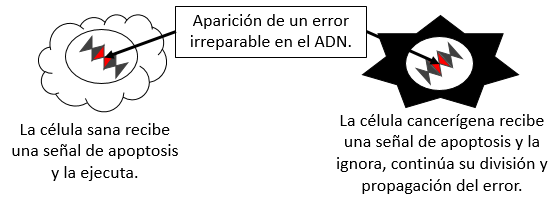
\includegraphics{img/fig-apoptosis.png}}
\end{center}\vspace*{-0.6cm}
\caption[Representaci\'on del proceso de apoptosis en una c\'elula sana y una cancer\'igena ante la aparici\'on de un error en el c\'odigo gen\'etico]{Representaci\'on del proceso de apoptosis en una c\'elula sana y una cancer\'igena ante la aparici\'on de un error en el c\'odigo gen\'etico \cite{viabarre2019}.}
\label{fig-apoptosis}
\end{figure}

\section{Angiogénesis}
\hspace{.1cm}Las células y los tejidos necesitan oxígeno y nutrientes para sobrevivir y proliferar por lo que la mayoría de las células yacen a menos de 0.1mm de un capilar sanguíneo. Bajo la mayoría de las circunstancias las células que conforman el endotelio, tejido que recubre la zona interna de todos los vasos sanguíneos y el corazón, no se dividen ni crecen. Sin embargo, bajo ciertas situaciones como la sanación de una herida, se activa la división de las células endoteliales provocando el crecimiento de nuevos capilares sanguíneos. Este proceso se conoce como angiogénesis o neovascularización.

\hspace{.1cm}Los tumores tienen la capacidad de inducir la angiogénesis y constituye un paso fundamental en la transición de un grupo pequeño de células mutadas (\textit{tumor in situ}) en un crecimiento maligno capaz de invadir los tejidos vecinos y órganos distantes. Esta transición puede tomar muchos meses o años, y a menos que se induzca la angiogénesis, los tumores sólidos no crecerán más de 1-2mm. Como ocurre con la mayoría de los mecanismos que mantienen la homeostasis celular, la angiogénesis también comprende un balance entre señales positivas y negativas que estimulan o inhiben este proceso. Se conoce que la habilidad para inducir y mantener la angiogénesis se adquiere en una serie de pasos discretos durante el desarrollo tumoral. Se muestra a continuación una revisión simplificada de este proceso [\cite{robins}, \cite{hanahan}, \cite{cancerbook}]:
\begin{itemize}
    \item El tumor libera factores angiogénicos que se difunden en los tejidos cercanos se acoplan a receptores en las células endoteliales de los vasos sanguíneos preexistentes, provocando su activación.
    \item Tales interacciones entre las células tumorales y las endoteliales conlleva a la secreción y activación de enzimas que degradan la membrana basal y la matriz extracelular.
    \item La degradación de la membrana basal permite que las células endoteliales activas migren hacia el tumor.
    \item Las células endoteliales depositan una nueva membrana basal y secretan factores de crecimiento que atraen a células de soporte de la matriz extracelular para que estabilicen el nuevo vaso sanguíneo.
\end{itemize}

Sin embargo, todavía no se comprenden por completo los mecanismos que afectan el balance angiogénico a favor del tumor. El escenario más probable es que existan relaciones entre estos mecanismos de balance y otros reguladores de la homeostasis celular. Por ejemplo, el gen supresor de tumores p53 se encuentra estrechamente relacionado con un inhibidor angiogénico. Por tanto, cualquier afectación al normal funcionamiento del gen p53, que es común en el desarrollo tumoral, puede causar una caída en los niveles del inhibidor provocando un desbalance angiogénico [\cite{robins}, \cite{hanahan}, \cite{cancerbook}].

\hspace{.1cm}La angiogénesis tumoral constituye un blanco irresistible para el desarrollo de terapias que afecten el desarrollo tumoral. En la actualidad los tratamientos antiangiogénicos constituyen una fracción numerosa de los ensayos clínicos que se están llevando a cabo para combatir el cáncer.

\section{Metástasis}
\hspace{.1cm}Los tumores sólidos, bajo condiciones óptimas, pueden invadir los tejidos locales y atravesar el sistema circulatorio para colonizar órganos y tejidos distantes. Estos tumores secundarios son responsables de casi el 90\% de las muertes relacionadas con el cáncer. La capacidad de las células tumorales de invadir y colonizar es la sexta marca distintiva del cáncer. Según [\cite{robins}, \cite{hanahan}], las definiciones de los términos invasión local y metástasis son:
\begin{itemize}
    \item \textbf{Invasión local}: El crecimiento del cáncer se acompaña de una infiltración, invasión y destrucción progresivas del tejido circundante, mostrando un rompimiento de la membrana basal. Además de las metástasis, la capacidad de invasión es el rasgo más fiable para distinguir el cáncer de los tumores benignos.
    \item \textbf{Metástasis}: Se define como la propagación del tumor a sitios físicamente alejados del tumor primario y marca, de un modo inequívoco, dicho tumor como maligno ya que por definición, una neoplasia benigna no metastatiza.
\end{itemize}

\hspace{.1cm}Una vez que un tumor infiltra satisfactoriamente los tejidos vecinos sanos, las células cancerígenas que lo conforman sufren distintas transformaciones que provocan la pérdida de la capacidad de adhesión celular y cambios en la matriz de interacción intercelular [\cite{hanahan}, \cite{cancerbook}]. La disminución de la adhesión celular permite que ocurran desprendimientos de células cancerígenas pertenecientes al tumor primario. Estas células sufren cambios en la matriz de interacción celular que provocan la expresión de proteínas involucradas en el control de la movilidad, la supresión de reguladores de la migración y la degradación de la ECM y la membrana basal. De esta forma pueden migrar a través del tejido circundante y adaptarse rápidamente para vencer numerosas dificultades que presentan los nuevos entornos [\cite{hanahan}, \cite{cancerbook}]. Estas células también son la causa fundamental de las recurrencias cuando la masa principal del tumor es removida quirúrgicamente \cite{kansal3}.

\hspace{.1cm}Las células cancerígenas muestran una variedad de estrategias de migración y pueden alternar entre ellas para hacerle frente a entornos hostiles [\cite{migration}]. Los factores determinantes en el proceso de migración son la expresión de mecanismos de unión intercelulares y los cambios de la estructura de las células invasivas. La invasión individual puede ser llevada a cabo por células con estructuras espigadas, elongadas y redondeadas [\cite{migration}] que degradan la matriz extracelular y se mueven a través de ella. La invasión colectiva puede darse en forma de conjuntos migrantes que se desprenden del tumor o formando largas cadenas invasivas que parten desde el mismo [\cite{robins}, \cite{hanahan}, \cite{cancerbook}].

\hspace{.1cm}Eventualmente las células migrantes entran en contacto con el sistema circulatorio, ya sea con capilares sanguíneos o vasos linfáticos. En este punto pueden penetrar dicho sistema, viajar en su interior hasta encontrar una localización favorable para abandonarlo y colonizar el tejido circundante. A este proceso se le conoce como metástasis y los pasos que la comprenden constituyen la cascada metastásica: invasión local, migración, penetración del sistema circulatorio (\textit{intravasation}), transporte, abandono del sistema circulatorio \textit{(extravasation}), formación de micrometástasis y colonización [\cite{robins}, \cite{invasion}, \cite{hanahan}, \cite{cancerbook}]. Una vez el tumor primario ha comenzado el proceso de angiogénesis, si bien las células cancerígenas deben tener las características necesarias para efectuar la invasión local, pueden acceder al sistema circulatorio desde los recién formados capilares sanguíneos que sustentan al tumor, sin la necesidad de penetrar los tejidos vecinos.
\hspace{.1cm}Las mutaciones necesarias para que las células cancerígenas sean capaces de efectuar la invasión local y la metástasis son comunes para ambos procesos. Sin embargo, para la colonización satisfactoria de un órgano distante estas células deben poseer una mayor resistencia. El proceso de metástasis es altamente ineficiente \cite{pubmed}, ya que la cantidad de células que dejan el tumor primario son del orden de los millones en un día, pero solo una pequeña fracción de las mismas son capaces de sobrevivir a la cascada metastásica. Las células migratorias pueden terminar su existencia por una gran variedad de causas, entre las que se encuentran:
\begin{itemize}
    \item Una célula sobrevive normalmente conectada a sus vecinos y al conjunto de proteínas existentes a su alrededor. El desprendimiento de la superficie de otras células puede llevar a la muerte celular.
    \item Las células cancerígenas son con frecuencia mucho mayores en tamaño que las células que viven en el sistema circulatorio. Cuando estas viajan a través de dicho sistema pueden dañarse o atascarse, llevando a la muerte celular.
    \item Las células cancerígenas pueden ser reconocidas y destruidas por células del sistema inmunitario.
\end{itemize}

\hspace{.1cm}Aún cuando una célula metastásica sobrevive todo el proceso, esto no significa que forme un tumor secundario satisfactoriamente. Dicha célula debe crear un entorno favorable dentro de un nuevo ambiente hostil que les permita sobrevivir y crecer. Esta capacidad de transformar el entorno es un hecho crucial como lo demuestran numerosos experimentos \cite{pubmed}. En un estudio experimental de un melanoma metastásico, más del 80\% de las células cancerígenas sobrevivieron al transporte a través del sistema circulatorio y arribaron al hígado. De estas, solamente 1 célula de cada 40 formaron micrometástasis en un lapso de 3 d\'ias, y 1 de cada 100 formaron macrometástasis en 10 días. La tarea de crear un entorno favorable parece ser un proceso complejo que limita notablemente la capacidad de la célula de formar un tumor secundario. Cuando una célula cancerígena entra en contacto con un nuevo órgano, puede ocurrir una de tres variantes:
\begin{itemize}
    \item El tejido circundante del nuevo órgano puede ser muy diferente de donde se originó el tumor primario, y en la mayoría de los casos puede ser muy hostil, al punto de impedir la supervivencia de la célula cancerígena, llevando a su muerte celular.
    \item Si dicha célula metastásica no posee la capacidad de transformar el tejido en un entorno más amistoso, no podrá colonizar satisfactoriamente. En este caso se dice que la célula entra en un período de dormancia, no muere, pero no es capaz de crecer. Ocasionalmente dichas micrometástasis latentes obtienen nuevas mutaciones que les permite colonizar satisfactoriamente dicho órgano.
    \item La célula migrante posee todas las capacidades necesarias para colonizar la nueva localización, como se ha comprobado en tumores que hacen metástasis en el mismo órgano donde surgió el tumor primario, o en órganos específicos. Distintos tipos de cáncer tienen preferencia por órganos específicos para ser atacados por células migratorias \cite{invasion}.
\end{itemize}

\hspace{.1cm}Precisamente la tendencia de colonizar órganos específicos según los diferentes tipos de cáncer se conoce como la hipótesis de la semilla y el sustrato (\textit{the seed and soil hypothesis}) \cite{paget}. En 1889 Stephen Paget observó que los pacientes con cáncer de mama desarrollaban tumores secundarios en el hígado con frecuencia. Consideró que era poco probable que esto sucediese principalmente por la accesibilidad del hígado al sistema circulatorio, ya que otros órganos que poseen un acceso al suministro de sangre equivalente desarrollaban metástasis muy rara vez. En base a esto, desarrolló dicha hipótesis, en la cual ciertas células cancerígenas solo pueden colonizar satisfactoriamente órganos selectos que poseen entornos de crecimiento adecuados o deseables [\cite{paget}, \cite{metastasis}], entre los que se incluye el entorno del órgano primario. Esta hipótesis comprende tres conceptos importantes:
\begin{itemize}
    \item Los tumores primarios y sus metástasis están compuestos de células tumorales genéticamente muy diversas.
    \item Las células seleccionadas para llevar a cabo la metástasis son las que pueden sobrevivir a toda la cascada.
    \item Las células seleccionadas colonizan una localización en una forma muy específica, y dado que los entornos de cada órgano son distintos las células cancerígenas solo podrán colonizar un tipo de órgano específico.
\end{itemize}

Estos conceptos muestran la idea de que una metástasis satisfactoria depende completamente de las interacciones entre las células cancerígenas y las células del órgano objetivo. Estas células que recién están formando una nueva metástasis no solo tienen que ser capaces de producir los factores requeridos por ellas para sobrevivir y crecer en el nuevo entorno, sino que el entorno del nuevo órgano tiene que ser capaz de responder a estas señales y actuar en consecuencia. Si la célula cancerígena se encuentra en un entorno muy inhóspito será imposible que una metástasis se forme satisfactoriamente \cite{metastasis}. Si una célula cancerígena sobrevive al transporte en el interior del sistema circulatorio y lleva a cabo la extravasación de forma satisfactoria puede ocurrir una de tres situaciones \cite{circulating}:
\begin{itemize}
    \item La extravasación de la célula ocurre en la localización del tumor donde se originó, es decir, penetró el sistema circulatorio, sobrevivió a su transporte y arribó al propio punto de origen. En este caso contribuye a la población tumoral en la localización primaria.
    \item La extravasación de la célula ocurre en la localización de una metástasis. En este caso se comporta de igual forma, contribuyendo con la población tumoral.
    \item La extravasación de la célula ocurre en una localización no colonizada aún. En este caso puede asentarse y comenzar una nueva metástasis.
\end{itemize}